\documentclass[letterpaper,superscriptaddress,aps,pra,nolongbibliography,twocolumn,showpacs,floatfix,10pt]{revtex4-2} % {{{
\usepackage{url}
\usepackage{amsmath}
\usepackage{amssymb}
\usepackage[utf8]{inputenc}
\usepackage[spanish]{babel}
\usepackage[T1]{fontenc}

\usepackage{ulem}

\usepackage{tikz}
\usetikzlibrary{arrows}


%\usepackage{slashbox}

\usepackage{amsmath}
\usepackage{hyperref}
\usepackage{lipsum}
\usepackage{graphicx,helvet}
\usepackage{color}
%\usepackage{bm}                      % added by TG
\usepackage{mathtools}
%\usepackage[inline]{showlabels}
%\usepackage[inner]{showlabels}
\usepackage{bbm,bm}
\usepackage{soul}
\usepackage{amsfonts}
 \usepackage{amsmath}
\usepackage{lipsum}% http://ctan.org/pkg/lipsum
\definecolor{mygray}{gray}{0.4}
\definecolor{light-blue}{rgb}{0.8,0.85,1}
\graphicspath{{images/}}
\usepackage{amsthm}
%\usepackage{MnSymbol}%
%\usepackage{wasysym}%
%\usepackage{bbm}% bold math
%\usetikzlibrary{decorations.shapes}
\usepackage[draft,inline,nomargin]{fixme} \fxsetup{theme=color}
\newcommand\dsone{\mathds{1}}
\FXRegisterAuthor{cp}{acp}{\color{blue}CP}
\FXRegisterAuthor{fl}{afl}{\color{orange}FL}
\definecolor{jacolor}{RGB}{200,40,0} \FXRegisterAuthor{ja}{aja}{\color{jacolor}JA}
\FXRegisterAuthor{dd}{ddg}{\color{green}DD}
\FXRegisterAuthor{af}{aaf}{\color{magenta}AF}

\newcommand{\esqueletoja}[1]{\textcolor{jacolor}{#1}}


\newcommand{\cuadritotikz}{
% \pgfmathsetmacro{\unitstep}{5.2}
% \node at (-0.5,0.5) {(a)} ;
    \foreach \x in {0,1,2,3} {
      \foreach \y in {0,1,2,3} {
        \begin{scope}[shift={(\x,-\y)}] 
          \draw[black!10] (0,0) rectangle (1,1); 
%           \node at (0.5,0.5) {$\tau_{\y,\x}$};
         \end{scope}
%         \node[block] at (2,-\y) (block\y) {$f_\y$};
%         \draw[->] (block\y.east) -- +(0.5,0);
    }
    }
 \draw (0,-3) rectangle (4,1);
}




\usepackage{color}
\usepackage{colortbl}
\usepackage{multirow}





\newcommand\todo[1]{\textcolor{red}{#1}}
% \renewcommand\todo[1]{}
%\def\>{\rangle} \def\<{\langle}
\renewcommand{\>}{\rangle}
\mathchardef\Re="023C
\mathchardef\Im="023D
%\usepackage[mathlines]{lineno}  
%\linenumbers
% \setlength\linenumbersep{3pt}%\modulolinenumbers[5]
% \newcommand{\red}{\color{red}}
\newcommand{\<}{\langle}
\newcommand{\mele}[2]{\ensuremath{| #1 \rangle \langle #2 |}}
\newcommand{\prj}[1]{\ensuremath{| #1 \rangle \langle #1 |}}
\newcommand{\jami}{Jamiołkowski}
\newcommand{\mcU}{\mathcal{U}}
\newcommand{\mcO}{\mathcal{O}}
\newcommand{\mcI}{\mathcal{I}}
\newcommand{\mcL}{\mathcal{L}}
\newcommand{\mcB}{\mathcal{B}}
\newcommand{\mcH}{\mathcal{H}}
\newcommand{\mcT}{\mathcal{T}}
\newcommand{\mcE}{\ensuremath{\mathcal{E}}}
\newcommand{\mcG}{\ensuremath{\mathcal{G}}}
\newcommand{\mcM}{\mathcal{M}}
\newcommand{\mcN}{\mathcal{N}}
\newcommand{\nnn}{\mathcal{N}}
\newcommand{\choi}{\ensuremath{\mcD}}
\newcommand{\mmm}{\mathcal{M}}
\newcommand{\sss}{\mathcal{S}}
\newcommand{\mcD}{\mathcal{D}}
\newcommand{\mcA}{\mathcal{A}}
\newcommand{\mcP}{\mathcal{P}}
\newcommand{\valpha}{{\vec \alpha}}
\newcommand{\one}{\openone}
\newcommand{\setA}{\ensuremath{{\sf A}}}
\newcommand{\hilbert}{\ensuremath{{\sf H}}}
\newcommand{\spV}{\ensuremath{V}}
\newcommand{\spW}{\ensuremath{W}}
\newcommand{\id}{\text{id}}
\newcommand{\pce}{\ensuremath{\text{PCE}}}
\newcommand{\vbeta}{\vec \beta}
\newcommand{\vlambda}{\vec \lambda}
\newcommand{\vtau}{\vec \tau}
\newtheorem{theorem}{Theorem}
\newtheorem{definition}{Definition}
\newtheorem{proposition}{Proposition}
\newtheorem{corollary}{Corollary}
\newtheorem{lemma}{Lemma}
\newcommand{\mcQ}{\mathcal{Q}}
% \newcommand{\mcG}{\mathcal{G}}
\newcommand{\mcF}{\mathcal{F}}
\newcommand{\mcK}{\mathcal{K}}
\newcommand{\mcS}{\mathcal{S}}
\newcommand{\ie}{i.e.}
\newcommand{\aka}{a.k.a}
\newcommand{\fmlong}{fuzzy measurements}
\newcommand{\Fmlong}{Fuzzy measurements}
\newcommand{\ipr}{\mathrm{ipr}}
\newcommand{\rmH}{\mathrm{H}}
\newcommand{\rmq}{\mathrm{q}}
\newcommand{\cut}{\mathrm{cut}}
\newcommand{\rmd}{\mathrm{d}}
\newcommand{\rmi}{\mathrm{i}}
\newcommand{\blue}{\color{blue}}
\newcommand{\mcC}{\mathcal{C}}
\newcommand{\cg}{\mcC}
%%%%CG commands
\newcommand{\Loc}[1]{\ensuremath{\Lambda_#1^\text{L}}}
\newcommand{\NoLoc}[1]{\ensuremath{\Lambda_{#1}^\text{NL}}}
\newcommand{\NoLoct}[1]{\ensuremath{\tilde{\Lambda}_{#1}^\text{NL}} }
\newcommand{\fuzzytwo}[1]{\ensuremath{\Lambda_#1^\text{fuzzy}}}
\newcommand{\cgtwo}[1]{\ensuremath{\Lambda_#1^\text{cg}}}
% \newcommand{\tp}{TP}
\newcommand{\hp}{HP}
\newcommand{\Imi}{\imath}
\newcommand{\rmf}{f}
%\newcommand{\eg}{\textit{e.g.} }
%\newcommand{\Eg}{\textit{E.g.} }
\newcommand{\eref}[1]{Eq.~(\ref{#1})} 
\newcommand{\sref}[1]{sec.~\ref{#1}}
\newcommand{\fref}[1]{fig.~\ref{#1}}
\newcommand{\tref}[1]{table~\ref{#1}}
\newcommand{\Eref}[1]{Eq.~(\ref{#1})} 
\newcommand{\Sref}[1]{Sec.~\ref{#1}}
\newcommand{\Fref}[1]{Fig.~\ref{#1}}  
\newcommand{\Tref}[1]{Tabla~\ref{#1}}
\newcommand{\Or}{\mathord{\mathrm{O}}}
\newcommand{\tr}{\mathop{\mathrm{Tr}}u\nolimits}
% \newcommand{\comm}[1]{{\color{red} #1 }}
\newcommand{\qv}{QV}
\newcommand{\old}{\infty}
\newcommand{\Mmed}{\mcM^{\<\cdot\>}}
\newcommand{\MBLP}{\mcM^{\text{BLP}}}
\newcommand{\MRHP}{\mcM^{\text{RHP}}}
\newcommand{\gs}{GS}
\newcommand{\cptp}{CPTP}
\newcommand{\ket}[1]{{\vert #1 \rangle}}
\newcommand{\bra}[1]{{\langle #1 \vert}}
\newcommand{\proj}[2]{{\vert #1 \rangle \langle #2 \vert}}
\newcommand{\projj}[1]{{\vert #1 \rangle \langle #1 \vert}}
% \newcommand{\cp}{\color{red}   }
\newcommand{\diag}{\text{diag}}

% --------------------------------------- Commands added by JA ------------------------------------
\usepackage{physics}
\usepackage{breqn}
% \newcommand{\paulicomponents}{r_{\alpha_1,\ldots,\alpha_N}}
\newcommand{\paulicomponents}{r_\valpha}
\newcommand{\taus}{\tau_\valpha}
\newcommand{\pceg}{\mcG_{\vec \alpha}}
\newcommand{\appref}[1]{appendix~\ref{#1}}
% 
\def\bbra#1{\mathinner{\langle \! \langle{#1}|}}
\def\kket#1{\mathinner{|{#1}\rangle \! \rangle}}
\def\ddyada#1{\mathinner{|{#1}\rangle\!\rangle\!\langle\!\langle{#1}|}}
\def\ddyad#1#2{\mathinner{|{#1}\rangle\!\rangle\!\langle\!\langle{#2}|}}
\def\bbrakket#1#2{\mathinner{\langle\!\langle {#1}|{#2}\rangle\!\rangle}}
% \newcommand{\R}[1]{\label{#1}\linelabel{#1}}
% \newcommand{\lr}[1]{\lineref{#1}}
% --------------------------------------------------------------------------------------------------------------

%\newcommand{\mimath}{\rmi}
%\newcommand{\into}{\int_0^t \rmd \tau \{\blue [Verbo de la introducción]}int_0^t \rmd \tau'}
%\newcommand{\intoh}{\int_0^t \rmd \tau \int_0^\tau \rmd \tau'}

%\providecommand{\openone}{\leavevmode\hbox{\small1\kern-3.8pt\normalsize1}}

%\newcommand{\eps}{\varepsilon} \newcommand{\trc}{\tr_{\rm c}}
%\newcommand{\tre}{\tr_{\rm e}} \newcommand{\mcH}{\mathcal{H}}
%\newcommand{\mcO}{\mathcal{O}} \newcommand{\mcU}{\mathcal{U}}

\newcommand{\shk}{Sherrington-Kirkpatrick}
\newcommand{\syr}{Šimkovic y Ross}

% }}}
\begin{document}
% Title, authors, etc {{{
\title{Monte Carlo de cadena de Markov de muchas configuraciones} 
\author{José Alfredo de León} 
\begin{abstract} % {{{
En este documento hacemos la propuesta de reproducir 
los resultados de un nuevo método de Monte Carlo
de cadena de Markov, propuesto por Šimkovic y Ross en
\cite{simkovic2021manyconfiguration}, aplicado al modelo de Sherrington-Kirkpatrick
y al modelo de Fermi-Hubbard.
\end{abstract} % }}}
%%
%\pacs{03.65.Yz, 03.65.Ta, 05.45.Mt}
 
\maketitle
% }}}

\section{Introducción e idea general}
Para el proyecto del curso de Métodos de Simulación Computacional de Sistemas
Cuánticos proponemos reproducir los resultados del artículo ``\textit{Many-configurations
Markov-Chain Monte Carlo}'' de Fedor Šimkovic y Riccardo Ross~\citep{simkovic2021manyconfiguration}.
En este artículo los \syr{} proponen una generalización del método de Monte
Carlo de cadena de Markov en el que el la configuración propuesta en 
cada paso Monte Carlo son una configuración de estados y no un sólo 
estado, como en el algoritmo original. De acuerdo con \syr{}, su nuevo
algoritmo, en comparación con el algoritmo de Monte Carlo tradicional 
y cuando la paralelización está disponible o es posible calcular un número
grande de configuraciones sesgadas a ningún costo computacional extra,
hace más eficiente el tiempo de termalización y presenta
una aceleración en el tiempo que le toma alcanzar un error
estocástico deseado; estas ventajas 

\section{Marco teórico}
\subsection{Método de Monte Carlo de cadenas de Markov}
%\janote{usar la \Fref{fig:mcmc_algorithm}}
El método de Monte Carlo de cadena de Markov es un algoritmo para generar
muestras de una distribución de probabilidad \cite{hammersley2013monte}. Este método
computacional, y sus variaciones, tienen muchas aplicaciones para
de sistemas cuánticos correlacionados \cite{becca2017quantum}.

El método de Monte Carlo de cadena de Markov (MCMC por sus siglas en inglés
``\textit{Markov-chain Monte Carlo}'') se basa en generar una secuencia 
de estados, tal que la probabilidad de transición entre los estados es markoviana,
es decir, depende sólo del estado actual. Por esta razón, recibe el nombre 
de Método de Monte Carlo de cadena de Markov. 
El objetivo del método MCMC es construir una cadena de estados de Markov 
tal que, para cada estado inicial, la probabilidad de un estado dado converja
a una distribución de probabilidad de equilibrio en el límite de tiempos muy 
grandes. El algoritmo se representa en la \Fref{fig:mcmc_algorithm}. En este algoritmo se propone, con una probabilidad arbitraria
$P(c_0|c_1)$ un estado nuevo $c_1$ dado el estado inicial $c_0$; luego
el estado propuesto $c_1$ es es aceptado o rechazado según una tasa 
que satisface el balance detalllado
\begin{align}
\text{min}\bigg( 1,\frac{P_{eq}(c_1)P_{prp}(c_0|c_1)}
{P_{eq}(c_0)P_{prp}(c_1|c_0)} \bigg),
\end{align}
conocida como tasa de Metrópolis. Despúes, se propone un nuevo estado 
$c_2$ ($c_1$) si se aceptó (rechazó) al estado $c_1$ y el algoritmo se repite.
Cada una de estas iteraciones es conocida como paso de Monte Carlo. 
En la siguiente sección describiremos un variación al método MCMC 
en el que, en cada paso de Monte Carlo, se propone una configuración de estados
$\{ c_i\}$ en vez de un sólo estado $c_1$.

\begin{figure}
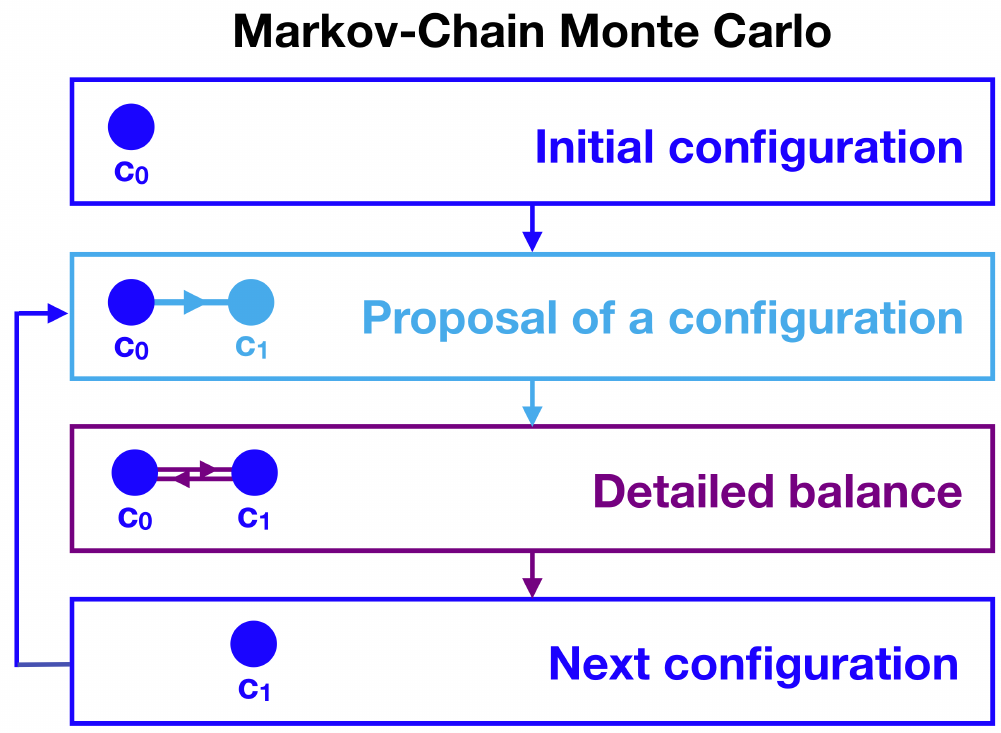
\includegraphics[width=0.7\columnwidth]{mcmc_algorithm}
\caption{Construcción de la cadena de Markov para el algoritmo 
estándar de Monte Carlo.
Se inicia en el estado $c_0$. Seguidamente se propone el estado $c_1$;
se hace el paso de Monte Carlo para aceptar o rechazar a $c_1$ y se repite
el proceso de proponer un nuevo estado.
Figura tomada de \cite{simkovic2021manyconfiguration}.}
\label{fig:mcmc_algorithm}
\end{figure}

\subsection{MCMCMC}
%\janote{describir la idea detrás del MCMCMC al cubo}
Ahora vamos a introducir el método de Monte Carlo de cadena de Markov
de muchas configuraciones (MCMCMC por sus siglas en inglés 
``\textit{Multi-configuration Markov-Chain Monte Carlo}''), 
propuesto por Šimkovic y Ross \cite{simkovic2021manyconfiguration}, 
como una generalización del método MCMC para muchas configuraciones. 
La idea básica del método consiste en proponer una configuración de muchos
estados en vez de uno sólo como se describe en la \Fref{fig:mcmcmc_algorithm}.
Supongamos que $c_0$ es el estado inicial de un paso Monte Carlo, entonces
proponemos una configuración de estados $\{ c_0,\ldots, c_5 \}$ como un grafo
dirigido, en donde la dirección del grafo entre los nodos $c_k$ y $c_j$ 
indica que el estado $c_j$ fue propuesto siguiendo la distribución de probabilidad
$P_{prp}(c_k|c_j)$. Luego, todos los nodos del grafo son visitados 
en un tiempo proporcional a la tasa a la que serían 
escogidos siguiendo la condición de equilibrio entre configuraciones
que pertenecen al mismo grafo pero ahora no dirigido. Luego de 
esta fase de termalización, se escoge un nodo con una probabilidad
proporcional a la tasa en la que el nodo es visitado y finalmente el 
proceso es iterado al siguiente paso de Monte Carlo. 

\begin{figure}
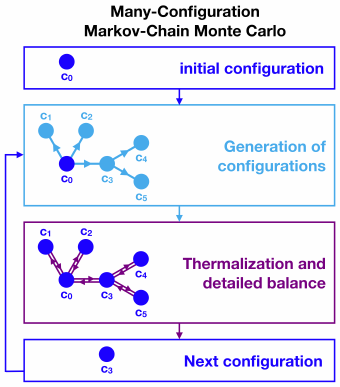
\includegraphics[width=0.7\columnwidth]{mcmcmc}
\caption{Construcción de la cadena de Markov para MCMCMC.
Se comienza con el estado inicial $c_0$. Seguidamente, se generan 
configuraciones $c_1,\ldots,c_5$, para luego pasar a la fase de termalización
en la que se utiliza una fracción del paso de Monte Carlo para visitar 
todos los nodos respetando el balance detallado. Finalmente, se escoge
el nuevo estado de la cadena de Markov del grafo con una tasa
que es igual a la fracción de tiempo transcurrida en cada nodo.
Figura tomada de \cite{simkovic2021manyconfiguration}.}
\label{fig:mcmcmc_algorithm}
\end{figure}

%\janote{no he dicho las ventajas del mcmcmc y las condiciones para usarlo}
Según \syr{} el método MCMCMC representa mejoras, en comparación con 
el método tradicional MCMC, en el tiempo de termalización y en la 
velocidad del algoritmo para alcanzar algún error estocástico deseado. 
El método MCMCMC supone que se tiene a disposición algunas de las 
siguientes dos opciones: (i) una computadora en la que se puede hacer
paralelización, o (ii) se pueden generar muchas configuraciones sesgadas
a poco o nulo gasto computacional extra. 
Ahora, en las siguientes dos secciones, vamos a discutir dos modelos
en los que podemos apreciar las ventajas que ofrece el método MCMCMC.

\subsection{El modelo de Sherrington-Kirkpatrick}\label{sec:Sh-k}
%\janote{meter las figs de la presentación}
El modelo de \shk{} fue introducido en 1975 como un modelo de vidrio de 
espín [vea \Fref{fig:shk} por David Sherrington y Scott Kirkpatrick \cite{panchenko2012sherrington}. 
Este es un modelo es Ising, en el que se consideran espines en una red, 
en el que se consideran acoplamientos ferro y antiferromagnéticas de largo alcance.
El Hamiltoniano para este sistema es  
\begin{align*}
H=\frac{1}{\sqrt{L}}\sum_{j\leq k}J_{jk}S_jS_k,
\end{align*}	
donde $L$ es el tamaño de la red, $S_j\in \{ -1, 1\}$ y $J_{jk}\in \mathbb{R}$
son números que siguen una distribución gaussiana con media igual a cero	
y varianza igual a uno.

En particular, para este trabajo nos interesará minimizar la energía promedio
por sitio, para lo cual se tiene la expresión
\begin{align}
\frac{\expval{E}}{L}=\frac{\sum_{\{S_j\}}e^{-H/T}H/L}{\sum_{\{S_j\}}e^{-H/T}},
\end{align}
que se calcula escribiendo la función de partición 
$\mathcal{Z}=\sum_{S_j}e^{-H/T}$ del sistema 
de espines y calculando la expresión $-d\mathcal{Z}/dT$. Debe mencionarse
que estamos considerando $k_B=1$.

\begin{figure}
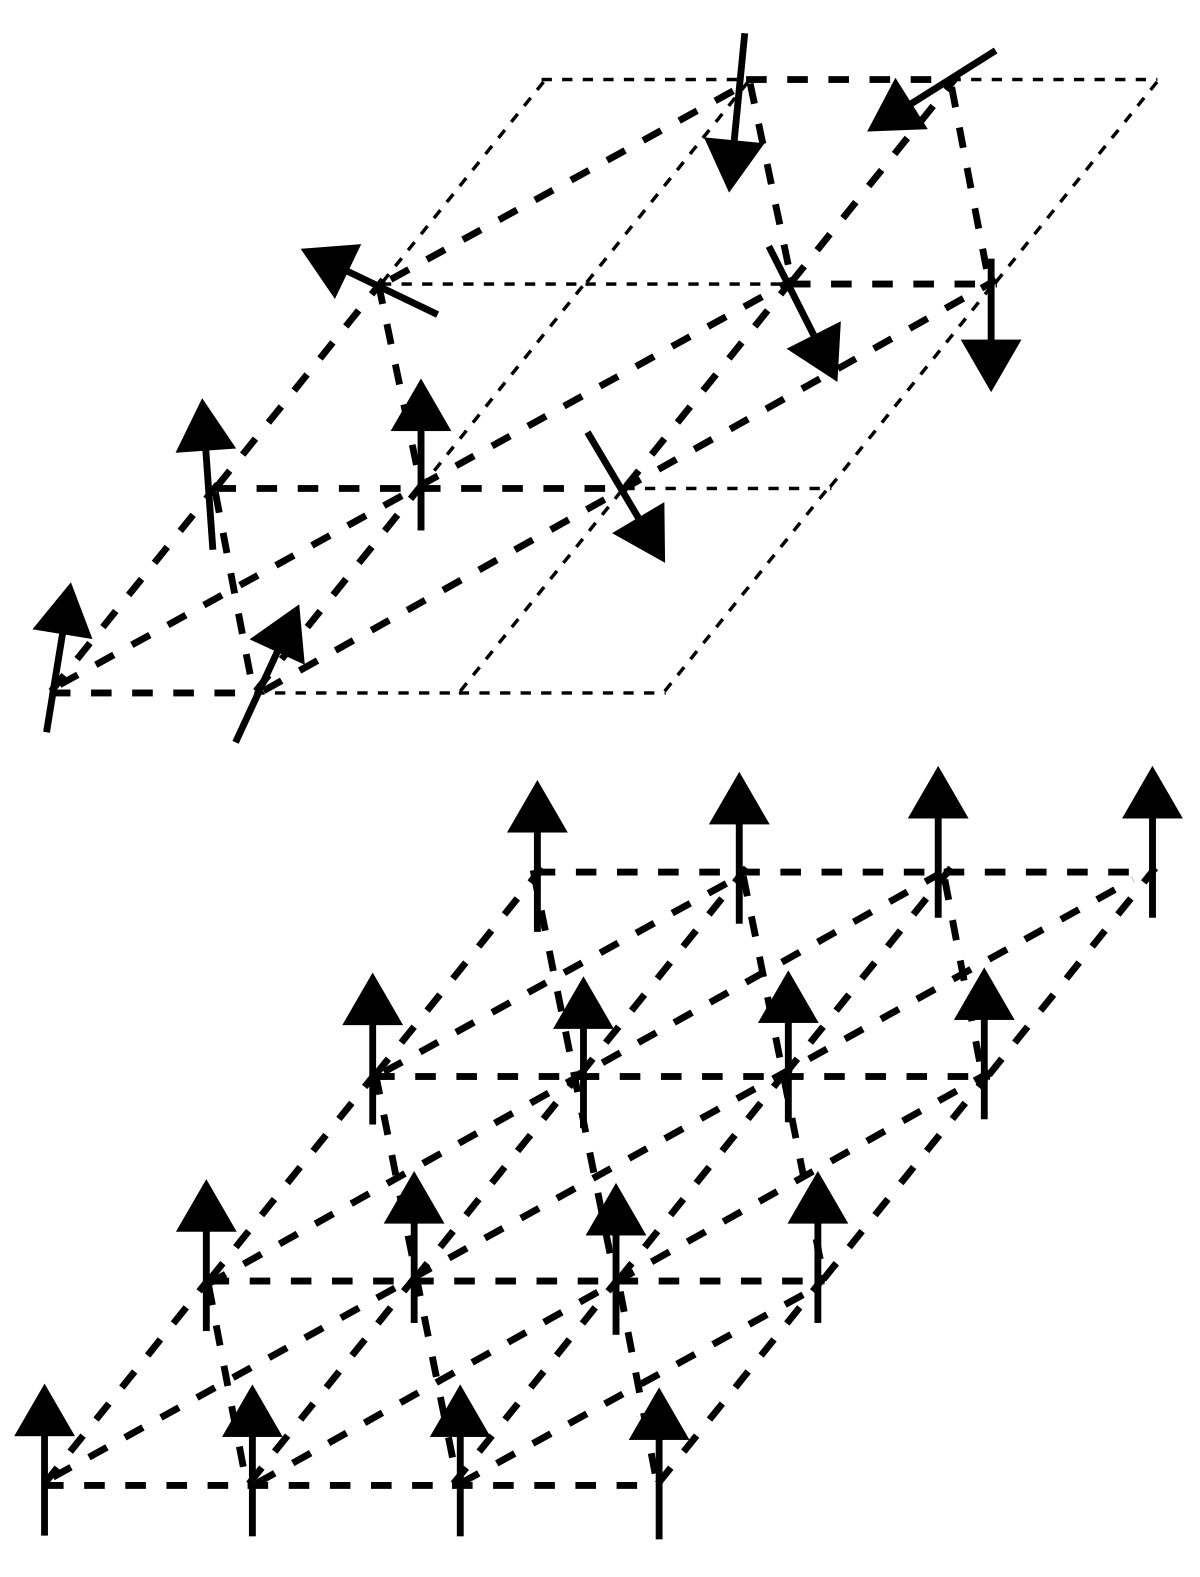
\includegraphics[width=0.5\columnwidth]{spin_glass}
\caption{Figura esquemática del modelo de Sherrington-Kirkpatrick. Tomada de Wikipedia.}
\label{fig:shk}
\end{figure}

\subsection{El modelo de Hubbard}\label{sec:Hub}
%\janote{describir qué es el modelo de fermi-hubbard}
El modelo de Hubbard [vea \Fref{fig:hubbard}] es un modelo de fermiones, propuesto por John Hubbard,
que interactúan en una red con dos términos en el Hamiltoniano: un término
cinético que permite el efecto túnel de las partículas entre los sitios de la red y un 
término de potencial asociado con la interacción entre espines en cada
sitio \cite{altland2006interaction}. Debe de destacarse que el trabajo 
orifinal de Hubbard fue un modelo para fermiones, sin embargo, trabajos
posteriores extendieron el modelo para partículas bosónicas.

Para este trabajo vamos a considerar el modelo de Hubbard dopado en una
red bidimensional, cuyo Hamiltoniano se escribe~\citep{simkovic2021manyconfiguration}
\begin{align}
H=\sum_{k,\sigma}(\epsilon_k-t 	)c_{k\sigma}^{\dagger}c_{k\sigma}
+
U\sum_{i}n_{\uparrow i}n_{i\downarrow},
\end{align}
con $\mu$ el potencial químico, $k$ el momentum, 
$\sigma\in \{\uparrow,\downarrow\}$ el espín, $U$ la magnitud de repulsión
en cada sitio, $i$ las etiquetas de cada sitio, y la dispersión $\epsilon_k$
está dada por
\begin{align}
\epsilon_k=-2t\qty[\cos(k_x) +\cos(k_y)],
\end{align}
donde $t$ es la amplitud de ``salto'' (\textit{hoping}) entre próximos vecinos.

\begin{figure}
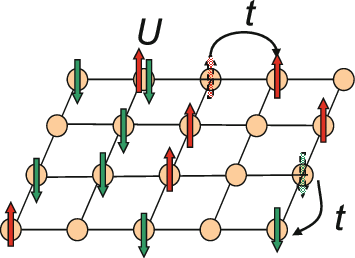
\includegraphics[width=0.7\columnwidth]{hubbard_model}
\caption{Figura esquemática del modelo de Hubbard. Tomada de \cite{10.1007/978-3-319-69953-0_14}.}
\label{fig:hubbard}
\end{figure}

\section{Objetivo}
%\janote{reproducir los resultados de los majes del paper. i.e.
%aplicar su nuevo método a los modelos y compararlo con el monte carlo 
%de cadena de markov}
Para este proyecto nos planteamos como objetivo principal 
reproducir los resultados del trabajo presentado por Šimkovic y Ross 
en \cite{simkovic2021manyconfiguration}, en el que se implementa una
variación del método de Monte Carlo de cadena de Markov, propuesta
por ellos mismos, aplicado a los modelos de Sherrington-Kirkpatrick y 
de Hubbard (para fermiones) para mostrar que su método supone mejoras en el
tiempo de termalización y el tiempo computacional que se necesita
para alcanzar algún error estocástico deseado.

Si bien el proyecto consiste en la resolución numérica de dos modelos físicos
la motivación para este proyecto es el aprendizaje de nuevas habilidades computacionales
para resolver problemas en la física, no sólo de métodos 
de Monte Carlo, sino también programación en paralela y la resolución 
de problemas frente a los obstáculos computacionales que puedan existir 
(y que casi siempre existen).

\section{Metodología}
%\janote{aquí que vayan los métodos?}
Para cumplir con el objetivo del proyecto
se proponen dos partes, una para estudiar los modelos físicos presentados 
en las secciones \ref{sec:Sh-k} y \ref{sec:Hub} y otra segunda parte para
realizar la implementación del método MCMC y MCMCMC para resolver 
ambos modelos y comparar con los resultados de las Figs. 7 y 8 de~\citep{simkovic2021manyconfiguration}.
A continuación, describimos con más detalle el trabajo a realizar en cada
una de las partes:

En la parte I deberá estudiarse con suficiente profundidad (a) el
método MCMCMC en el manuscrito de \syr{} \cite{simkovic2021manyconfiguration},
(b) el modelo de Sherrington-Kirkpatrick en la referencia \cite{panchenko2012sherrington};
y (c) el modelo de Hubbard en la referencia \cite{hirsch1985two}. Proponemos un estudio
profundo, más no exhaustivo, de los modelos físicos, pues no debemos de 
desviarnos del objetivo principal de este proyecto que es la tarea de la 
implementación computacional. En el manuscrito final del proyecto se deberá
incluir un resumen con las ideas más importantes de la revisión bibliográfica
sobre del método MCMCMC y de los modelos de Sherrington-Kirkpatrick y de Hubbard.

En la parte II se deberá implementar el método MCMC y MCMCMC y aplicarlos
a los dos modelos físicos. Se propone comenzar con una implementación en 
Mathematica de ambos métodos aplicados al modelo de Sherrington-Kirkpatrick
y reproducir los resultados de la Fig. 7 en \cite{simkovic2021manyconfiguration}.
Con esto pretendemos familiarizarnos con el método en un lenguaje que 
permite una implementación más rápida y práctica que en lenguajes como C/C++
o FORTRAN. Según la eficiencia y el costo computacional de la implementación
en Mathematica deberá tomarse una decisión si deberá o no implementarse
alguno de los dos o ambos métodos en FORTRAN para trabajar con el modelo 
de Hubbard. Se deberán reportar los resultados en el manuscrito final, así 
como las dificultades enfrentadas durante la parte II, si las hubiere. 


\section{Cronograma} % {{{
Para cumplir con el trabajo se proponen tareas específicas y un cronograma 
para seguir durante el desarrollo del proyecto. Primero enlistamos las tareas
específicas a continuación. 
\begin{itemize}
\item Tarea 1: Estudiar el algoritmo de Monte Carlo de cadena de Markov 
de muchas configuraciones del propio trabajo de \syr{} en \cite{simkovic2021manyconfiguration}.
\item Tarea 2: Estudiar el modelo de Sherrrington-Kirkpatrick en \cite{panchenko2012sherrington}.
\item Tarea 3: Estudiar el modelo de Fermi-Hubbard en \cite{hirsch1985two,white1989numerical}.
\item Tarea 4: Escribir un resumen con el compilado de las ideas del MCMCMC
y los dos modelos físicos en el manuscrito final del proyecto.
\item Tarea 5: Realizar la implementación del MCMC para resolver el modelo
de Sherrington-Kirkpatrick en Mathematica.
\item Tarea 6: Realizar la implementación del MCMCMC para resolver el modelo
de Sherrington-Kirkpatrick en Mathematica.
\item Tarea 7: Preparar presentación del avance del proyecto.
\item Tarea 8: (por decidir) Realizar la implementación en lenguaje no interpretado
del MCMC para resolver el modelo de Hubbard o resolverlo utilizando la 
implementación en Mathematica.
\item Tarea 9: Escribir los resultados y discusión del trabajo en el manuscrito
final del proyecto. 
\item Tarea 10: Preparar la presentación final de los resultados del proyecto.
\end{itemize}

En la \Tref{tab:cronograma} mostramos el cronograma de tareas propuesto. 
El cronograma de actividades se propone de tal manera que para la fecha de
presentación del avance del proyecto se haya reproducido (tenido problemas con)
el primer resultado de \cite{simkovic2021manyconfiguration}.

\begin{table}[]
%\begingroup
%\setlength{\tabcolsep}{2pt} % Default value: 6pt
%\renewcommand{\arraystretch}{1} % Default value: 1
\centering
\resizebox{\columnwidth}{!}{%
\begin{tabular}{|l|l|l|l|l|l|l|l|l|l|l|l|l|l|l|l|}
\hline
   & S8 & S9 & S10 & S11 & S12 & S13 & S14 & S15 & S16 & S17 & S18 & S19 & S20 & S21 & S22 \\ \hline
T1 &  \cellcolor[gray]{0.5}  & \cellcolor[gray]{0.5}   &     &     &     &     &     &     &     &     &     &     &     &     &     \\ \hline
T2 &    &  \cellcolor[gray]{0.5}  &  \cellcolor[gray]{0.5}   &     &     &     &     &     &     &     &     &     &     &     &     \\ \hline
T3 &    &  \cellcolor[gray]{0.5}  &   \cellcolor[gray]{0.5}  &     &     &     &     &     &     &     &     &     &     &     &     \\ \hline
T4 &    &    &  \cellcolor[gray]{0.5}   &  \cellcolor[gray]{0.5}   &     &     &     &     &     &     &     &     &     &     &     \\ \hline
T5 &    &    &    &  \cellcolor[gray]{0.5}   &  \cellcolor[gray]{0.5}  &    &     &     &     &     &     &     &     &     &     \\ \hline
T6 &    &    &    &   \cellcolor[gray]{0.5}  &  \cellcolor[gray]{0.5}   &  \cellcolor[gray]{0.5}   &   \cellcolor[gray]{0.5}  &     &     &     &     &     &     &     &     \\ \hline
T7  &    &    &     &     &     &     &     &  \cellcolor[gray]{0.5}   &     &     &     &     &     &     &     \\ \hline
T8 &    &    &     &     &     &     &     &  \cellcolor[gray]{0.5}   &  \cellcolor[gray]{0.5}   &  \cellcolor[gray]{0.5}   &  \cellcolor[gray]{0.5}   &  \cellcolor[gray]{0.5}   &     &     &     \\ \hline
T9 &    &    &     &     &     &     &     &  \cellcolor[gray]{0.5}   &     &     &     &  \cellcolor[gray]{0.5}   &  \cellcolor[gray]{0.5}   &   \cellcolor[gray]{0.5}  &  \cellcolor[gray]{0.5}   \\ \hline
T10  &    &    &     &     &     &     &     &     &     &     &     &     &     &     &  \cellcolor[gray]{0.5}   \\ \hline
\end{tabular}
}
\caption{Cronograma de trabajo propuesto. Las columnas representan las semanas
del año. La semana 8 comienza el lunes 21 de febrero. Las filas representan las 
tareas. Los cuadros pintados indican las semanas en las que se debe de trabajar
cada tarea.}
\label{tab:cronograma}
%\endgroup
\end{table}

\bibliographystyle{unsrt}
\bibliography{references}

\end{document}
